\section{Производительность решения}

Целями следующих экспериментов является выявление эффекта произведеного использованием нескольких глобальных очередей и сопостовлением этих результатов с результатами использования нескольких рантаймов.

\subsection{Ход исследования}

Сценарий предоставленный командой \verb|TATLIN.BACKUP| был использова для измерния пропускной способности системы состоящей из нескольких рантаймов и одного рантайма с несколькими глобальными очередями, что представленно на рисунке~\ref{fig:tatlin:multi_rt_gp:eval}.

\begin{figure}[H]
    \begin{center}
        \makebox[\textwidth]{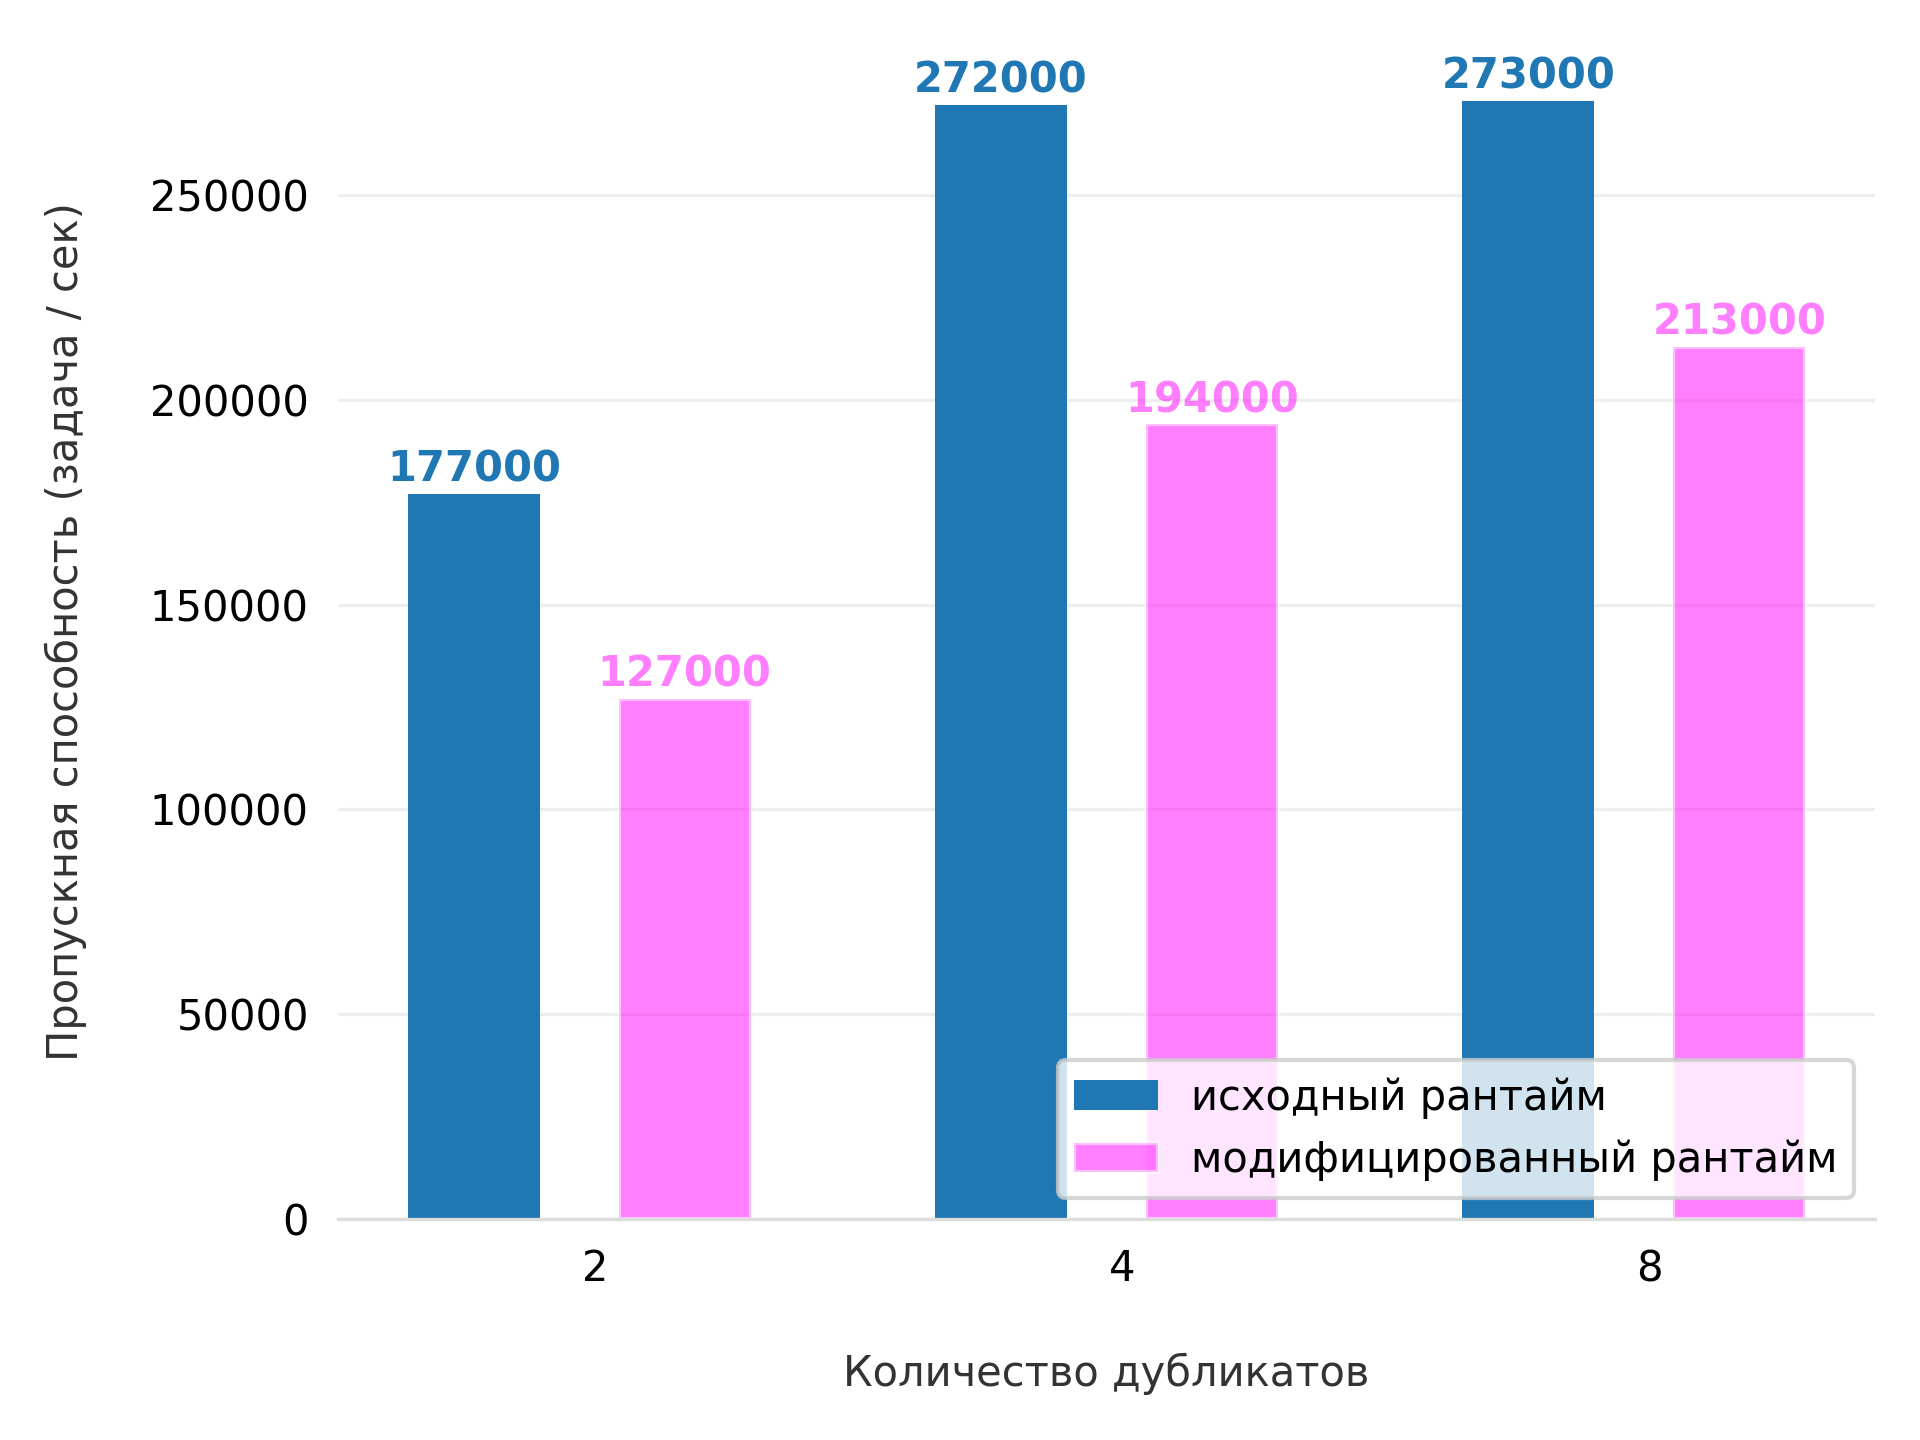
\includegraphics[scale=0.80]{pictures/rt_gp_nsapwner128_nspawn1000.png}}
    \end{center}

    \caption{Производительность системы при использовании нескольких рантаймов}
    \label{fig:tatlin:multi_rt_gp:eval}
\end{figure}

\subsection{Вывод}

\begin{itemize}
    \item Пропускная способность системы из одного рантайма и одного модифицированного рантайма содержащего одну глобальную очередь демонстрируют одинаковую пропускную способность.
    \item При увеличении количества глобальных очердей в системе состящей из одного рантайма наблюдается увеличение пропускной способности. Это ожидаемый результат:
    \begin{itemize}
        \item Меньшее количество воркеров конкурируют из глобальную очередь.
        \item Меньшее количество воркеров пытаются похитить задачи.
    \end{itemize}
    \item Пропускная способность системы состоящей из одного модицированного рантайма содержащего несколько очередей меньше пропускной способности системы состоящей из нескольких рантаймов. Это ожидаемый результат --- в системе состоящей из отдельных рантаймов требуется меньшее количество синхронизаций:
    \begin{itemize}
        \item Различные метрики собираемые рантаймом реализованы с помощью атомарных счетчиков, разделяемых в случае одного рантайма.
        \item Многие структуры данных находятся близко в памяти, что может так же потребовать дополнительной синхронизации между различными процессорами.
    \end{itemize}
\end{itemize}
